A Support Vector Machine(SVM) is a classifier which outputs an optimal hyperplane or set of hyperplanes in high-dimensional space and classifies new examples. In other words, SVM is a supervised learning model that employs learning algorithms to recognize patterns and analyze data, used for classification of unknown data\cite{wiki:SVM}.\\
In figure \ref{fig:SVM} main idea behind SVM is shown. Consider example dataset described by variables $x_1$ and $x_2$. The operation of SVM algorithm is based on finding the optimal hyperplane between training examples. An optimal hyperplane is one that gives the largest minimum distance to the training examples and it maximizes the margin between the hyperplane and all data points\cite{opencv_library}.

\begin{figure}[H]
    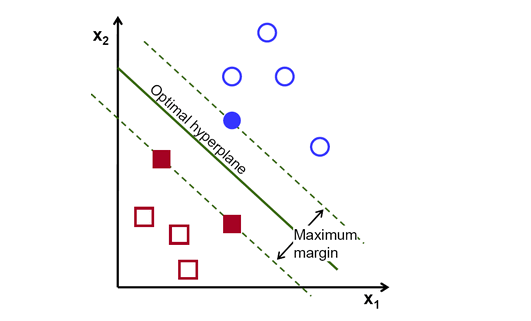
\includegraphics[width=80mm]{./img/SVM.png}
     \caption{Optimal Separating Hyperplane}
    \label{fig:SVM}
\end{figure}

In recent years, SVMs are widely used in bio-informatics \cite{furey2000support,osuna1997training,guyon2002gene} and other discipline due to its ability to accurately deal with high dimensional data\cite{joachims1998text}. They are popular for couple of theoretical reasons: SVMs are robust to very large number of variables and can learn both simple and complex classification models\cite{cristianini2000}.\\

SVMs is a best known member in the general category of kernel methods\cite{shawe2004kernel}. A kernel method has the ability to generate non-linear decision boundaries by using method designed for linear classifiers; This allows the user to apply a classifier to data that has infinite- dimensional vector space representation such as DNA or protein\cite{ben2010user}.    




